\section{Редукция обратной задачи к вариационной постановке}

Найдём решение задачи (\ref{eqn:direct_problem_1}), (\ref{eqn:direct_problem_2}), используя подход, описанный в \cite[Гл.~4,~\S~4]{tikh}.

Рассмотрим сперва случай одного источника: $\vect{v} = (x_1,y_1,z_1)$. Обозначим $M_1= (x_1,y_1,z_1)$ точку, в которой он расположен; начало координат обозначим $O$ (см. рис.~\ref{fig:source_func}).

\begin{figure}[h]
	\centering
	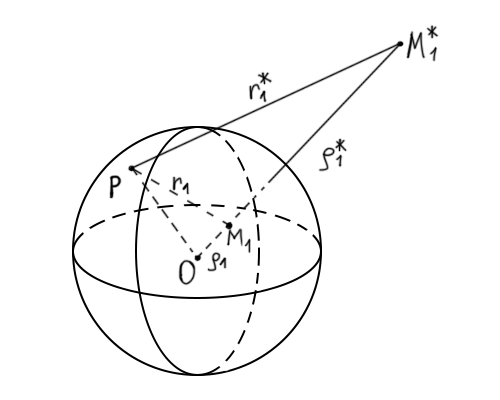
\includegraphics[scale=2]{sphere}
	\caption{Метод электростатических изображений}
	\label{fig:source_func}
\end{figure}

Воспользуемся методом функции источника: построим функцию
\begin{equation}
	G(M; M_1) = \frac{1}{ r_1} + v(M; M_1)\text{,}
\end{equation}
где $M$ --- произвольная точка из $T + \Sigma$, $r_1$ - расстояние между $M$ и $M_1$, $v$ --- некоторая гармоническая функция, непрерывная (по координатам т. $M$) в $T + \Sigma$ вместе с первыми производными, не имеющая в этом шаре особенностей и такая, что
\begin{equation}
	v\big|_\Sigma=-\frac{1}{ r_1}\text{.}
\end{equation}

Для построения воспользуемся методом электростатических изображений. Отложим на луче $OM_1$ точку $M_1^*$ такую, что
\[
OM_1 \cdot OM_1^* = 1\text{.}
\]
$M_1^*$ есть не что иное, как точка, сопряжённая с $M_1$ относительно сферы единичного радиуса с центром в начале координат.

Обозначим $\rho_1 = OM_1$ и $\rho_1^* = OM_1^*$; таким образом,
\[
\rho_1 \cdot \rho_1^* = 1\text{.}
\]

Покажем, что расстояния от всех точек $P$ поверхности сферы до $M_1$ и $M_1^*$ пропорциональны. Обозначим $r_1^*$ расстояние от $P$ до $M_1^*$.

Рассмотрим треугольники $OPM_1$ и $OPM_1^*$. Заметим, что
\[
\frac{OM_1}{OP} = \frac{OP}{OM_1^*}\text{,}
\]
и что угол при вершине $O$ - общий. Следовательно, эти треугольники подобны.

Подобие сторон
\[
\frac{OM_1}{OP} =
\frac{OP}{OM_1^*} =
\frac{PM_1}{PM_1^*}
\]
можно переписать в виде
\begin{equation}
	\frac{\rho_1}{1} =
	\frac{1}{\rho_1^*} =
	\frac{r_1}{r_1^*}\text{.}\label{proportion}
\end{equation}

Из последней пропорции следует, что
\[
r_1 = \rho r_1^*\text{,}
\]
а, значит, в качестве функции $v$ можно взять
\begin{equation}
	v(M; M_1) = - \frac{1}{ \rho_1 r_1^*}\text{.}
\end{equation}

Функция $G$ тогда принимает вид:
\begin{equation}
	G(M;M_1) =
	% \frac{1}{4 \pi}
	% \bigg(
	\frac{1}{r_1} -
	\frac{1}{\rho_1 r_1^*}
	% \bigg)
	\text{.}
\end{equation}

Полученная функция есть потенциал, создаваемый в точке $M$ единичным точечным зарядом, расположенным в точке $M_1=(x_1,y_1,z_1)$, при условии заземления поверхности сферы, т.е. решение прямой задачи (\ref{eqn:direct_problem_1}), (\ref{eqn:direct_problem_2}) для случая $\vect{v}=(x_1,y_1,z_1)$:
\begin{equation}
	u(x,y,z; \vect{v}) = 
	% \frac{1}{4 \pi}
	% \bigg(
	\frac{1}{r_1(x,y,z)} -
	\frac{1}{\rho_1 r_1^*(x,y,z)}
	% \bigg)
	\text{.}\label{eqn:potential_1}
\end{equation}

Найдём теперь нормальную производную этого потенциала на поверхности сферы. Из~(\ref{eqn:potential_1}):
\begin{equation}
	\frac{\partial u}{\partial n}
	=
	% \frac{1}{4 \pi}
	% \Bigg(
	\frac{\partial}{\partial n}
	\Big(
	\frac{1}{r_1}
	\Big)
	- \frac{1}{\rho_1}
	\frac{\partial}{\partial n}
	\Big(
	\frac{1}{r_1^*}
	\Big)
	% \Bigg)
	\text{.}\label{eqn:derivative_1}
\end{equation}

Производные по направлению внешней нормали $\mathbf{n}$ к сфере:
\begin{equation}
	\begin{aligned}
		&\frac{\partial}{\partial n}
		\Big(
		\frac{1}{r_{1}}
		\Big)
		=
		\frac{\partial}{\partial r_{1}}
		\Big(
		\frac{1}{r_{1}}
		\Big)
		\frac{\partial r_{1}}{\partial n}
		=
		-\frac{1}{r_{1}^2}
		\cos{(\widehat{\mathbf{r_{1}}, \mathbf{n}})}
		\text{,}\\[20pt]
		&\frac{\partial}{\partial n}
		\Big(
		\frac{1}{r_{1}^*}
		\Big)
		=
		\frac{\partial}{\partial r_{1}^*}
		\Big(
		\frac{1}{r_{1}^*}
		\Big)
		\frac{\partial r_{1}^*}{\partial n}
		=
		-\frac{1}{(r_{1}^*)^2}
		\cos{(\widehat{\mathbf{r_{1}^*}, \mathbf{n}})}
		\text{.}
		\label{partials}
	\end{aligned}
\end{equation}

Выразим направляющие косинусы через известные величины (см. рис. (\ref{fig:source_func})):
\begin{empheq}{align}
	&\cos{(\widehat{\mathbf{r_{1}}, \mathbf{n}})}
	=
	\frac{1 + r_{1}^2 - \rho_{1}^2}{2r_{1}}
	\text{,}\label{cos_1}\\[10pt]
	&\cos{(\widehat{\mathbf{r_{1}^*}, \mathbf{n}})}
	=
	\frac{1 + (r_{1}^*)^2 - (\rho_{1}^*)^2}{2r_{1}^*}
	\text{.}\label{cos_2}
\end{empheq}

Воспользуемся пропорциональностью (\ref{proportion}) и преобразуем (\ref{cos_2}):
\begin{equation}
	\cos{(\widehat{\mathbf{r_{1}^*}, \mathbf{n}})}
	=
	\cfrac{1 + \cfrac{r_{1}^2}{\rho_{1}^2} - \cfrac {1}{\rho_{1}^2}} {\cfrac{2 r_{1}}{\rho_{1}}}
	=
	\frac{\rho_{1}^2 + r_{1}^2 - 1}{2\rho_{1}r_{1}}
	\text{.}\label{cos_2_new}
\end{equation}

Полученные выражения для производных (\ref{partials}) и для косинусов (\ref{cos_1}), (\ref{cos_2_new}) подставим в исходное выражение (\ref{eqn:derivative_1}) для производной потенциала:
\begin{equation}
	\begin{split}
		\frac{\partial u}{\partial n}
		&=
		% \frac{1}{4 \pi}
		% \bigg[
		-\frac{1}{r_{1}^2}
		\cdot
		\frac{1 + r_{1}^2 - \rho_{1}^2}{2r_{1}}
		+
		\frac{\rho_{1}^2}{r_{1}^2}
		\cdot
		\frac{1}{\rho_{1}}
		\cdot
		\frac{\rho_{1}^2 + r_{1}^2 - 1}{2\rho_{1}r_{1}}
		% \bigg]
		=\\[10pt]
		&=
		% \frac{1}{4 \pi}
		% \cdot
		\frac{-(1 + r_{1}^2 - \rho_{1}^2) + \rho_{1}^2 + r_{1}^2 - 1}{2r_{1}^3}
		=\\[10pt]
		&=
		-
		% \frac{1}{4 \pi}
		% \cdot
		\frac{1 - \rho_{1}^2}{r_{1}^3}
		=\\[10pt]
		&=
		-
		% \frac{1}{4 \pi}
		% \cdot
		\frac{1 - x_1^2 - y_1^2 - z_1^2}
		{
			\big[
			(x - x_1)^2 + (y - y_1)^2 + (z - z_1)^2
			\big]^{\tfrac{3}{2}}}
		\text{.}\label{eqn:derivative_long_1}
	\end{split}
\end{equation}

Итак, получена нормальная производная потенциала в декартовых координатах для случая $\vect{v}=(x_1,y_1,z_1)$:
\begin{equation}
	\begin{split}
		\frac{\partial u}{\partial n}
		\Big|_\Sigma
		=
		-
		% \frac{1}{4 \pi}
		% \cdot
		\frac{1 - x_1^2 - y_1^2 - z_1^2}
		{
			\big[
			(x - x_1)^2 + (y - y_1)^2 + (z - z_1)^2
			\big]^{\tfrac{3}{2}}}
		\text{.}\label{eqn:normal_derivative_1}
	\end{split}
\end{equation}

В силу линейности задачи (\ref{eqn:direct_problem_1}), (\ref{eqn:direct_problem_2}) и оператора нормальной производной потенциал и его нормальная производная на поверхности $\Sigma$ в случае $N$ источников
\[
\vect{v}=(x_1,y_1,z_1,...,x_N,y_N,z_N)
\]
есть сумма полученных выше выражений для одного источника с соответствующей заменой индексов.

Таким образом, \textbf{решение задачи (\ref{eqn:direct_problem_1}), (\ref{eqn:direct_problem_2}) в случае $\vect{v}$ --- $3N$-мерного вектора}:
\begin{equation}
	u(x,y,z; \vect{v}) =
	% \frac{1}{4 \pi}
	\sum\limits_{i = 1}^{N}
	\bigg(
	\frac{1}{r_i(x,y,z)} -
	\frac{1}{\rho_i r_i^*(x,y,z)}
	\bigg)
	\label{eqn:potential}
\end{equation}
и его \textbf{нормальная производная на поверхности $\Sigma$}:
\begin{equation}
	\begin{split}
		\frac{\partial u}{\partial n}
		\Big|_\Sigma
		=
		-
		% \frac{1}{4 \pi}
		\sum\limits_{i = 1}^{N}
		\frac{1 - x_i^2 - y_i^2 - z_i^2}
		{
			\big[
			(x - x_i)^2 + (y - y_i)^2 + (z - z_i)^2
			\big]^{\tfrac{3}{2}}}
		\text{.}\label{eqn:normal_derivative}
	\end{split}
\end{equation}

Перейдём от вектора $\vect{v}$ к вектору $\vect{w}=\vect{w}(\vect{v}) \in \mathbb{R}^{3N}$, задающему ту же совокупность источников, но в сферических координатах. Cоответствующие преобразования координат:
\begin{equation}
	\begin{aligned}
		\rho_i
		&= 
		\sqrt{
			x_i^2 + y_i^2 + z_i^2
		}
		&\text{, }
		i=\overline{1,N}
		\text{,}
		\\[10pt]
		\phi_i
		&=
		\begin{cases}
			\begin{aligned}
				&\arctg{\frac{y_i}{x_i}}\text{, } x_i > 0\text{, } y_i > 0 \text{,}\\[5pt]
				&\arctg{\frac{y_i}{x_i}} + \pi \text{, } x_i < 0 \text{,}\\[5pt]
				&\arctg{\frac{y_i}{x_i}} + 2 \pi\text{, } x_i > 0\text{, } y_i < 0 \text{,}\\
			\end{aligned}
		\end{cases}
		&\text{, }
		i=\overline{1,N}
		\text{,}
		\\[10pt]
		\theta_i
		&=
		\arccos{
			\frac{z_i}
			{
				\sqrt{x_i^2 + y_i^2 + z_i^2}
		}}
		&\text{, }
		i=\overline{1,N}
		\text{.}
	\end{aligned}
\end{equation}

Обратные преобразования:
\begin{equation}
	\begin{aligned}
		x_i
		&=
		\rho_i \cos{\phi_i} \sin{\theta_i}
		&\text{, }
		i=\overline{1,N}
		\text{,}
		\\[10pt]
		y_i
		&=
		\rho_i \sin{\phi_i} \sin{\theta_i}
		&\text{, }
		i=\overline{1,N}
		\text{,}
		\\[10pt]
		z_i
		&=
		\rho_i \cos{\theta_i}
		&\text{, }
		i=\overline{1,N}
		\text{.}
	\end{aligned}
\end{equation}

Таким образом, ($\rho_i, \phi_i, \theta_i$) --- $i$-ый источник из $\vect{w}(\vect{v})$. Далее иногда для краткости будем писать просто~$\vect{w}$.

Введём в новых координатах обозначение для нормальной производной на поверхности сферы:
\begin{equation}
	\begin{split}
		g(\phi, \theta; \vect{w}) &=
		\frac{\partial u}{\partial n}
		\Big|_\Sigma =\\[10pt]
		&=
		-
		% \frac{1}{4 \pi}
		\sum_{i = 1}^{N} \frac{1 - \rho_i^2}
		{
			\big[
			1 + \rho_i^2 - 2\rho_i
			(cos(\phi - \phi_i)\sin\theta \sin\theta_i + \cos\theta \cos\theta_i
			)
			\big]^{\tfrac{3}{2}}}
	\end{split}
\end{equation}

Для сокращения записи введём \textbf{вспомогательную функцию}:
\begin{equation}
	K_i(\phi, \theta; \vect{w}) = 1 + \rho_i^2 - 2\rho_i(cos(\phi - \phi_i)\sin\theta \sin\theta_i + \cos\theta \cos\theta_i)\text{, }i=\overline{1,N}\text{,}
\end{equation}
тогда \textbf{нормальная производная} приобретает более компактный вид:
\begin{equation}
	\begin{split}
		g(\phi, \theta; \vect{w}) =
		\frac{\partial u}{\partial n} \Big|_\Sigma =
		-
		% \frac{1}{4 \pi}
		\sum_{i = 1}^{N}
		\frac{1 - \rho_i^2}
		{(K_i(\phi, \theta; \vect{w}))^{\tfrac{3}{2}}}
	\end{split}
\end{equation}

Сформулируем \textbf{вариационную постановку обратной задачи 1}.

Пусть на поверхности сферы известна нормальная производная $Q(\phi, \theta)$.

Требуется найти расположение источников $\vect{v}$, доставляющее минимум функции $\Phi$:
\begin{align}
	\Phi(\vect{w}(\vect{v}); Q) =
	\int\limits_{0}^{2\pi}\int\limits_{0}^{\pi}
	\big[g(\phi, \theta; \vect{w}(\vect{v})) - Q(\phi,\theta)\big]^2 
	\sin{\theta} \, d\phi \, d\theta \text{, }
	\rho_i < 1\text{, }
	i=\overline{1,N}
	\text{.}
\end{align}

\newpage
Сформулируем \textbf{вариационную постановку обратной задачи 2}.

Пусть часть поверхности сферы $\Sigma_1$ определяется следующим образом:
\begin{equation}
	\Sigma_1 = \{(\rho,\phi,\theta): \rho=1\text{, }
	\phi_1 \le \phi \le \phi_2\text{, }
	\theta_1 \le \theta \le \theta_2 \}\text{.}
\end{equation}


На $\Sigma_1$ известна нормальная производная $Q(\phi, \theta)$. Требуется найти расположение источников $\vect{v}$, доставляющее минимум функции $\Phi_{\Sigma_1}$:
\begin{align}
	\Phi_{\Sigma_1}(\vect{w}(\vect{v}); Q) =
	\int\limits_{\phi_1}^{\phi_2}
	\int\limits_{\theta_1}^{\theta_2}
	\big[g(\phi, \theta; \vect{w}(\vect{v})) - Q(\phi,\theta)\big]^2 
	\sin\theta \, d\phi \, d\theta \text{, }
	\rho_i < 1\text{, }
	i=\overline{1,N}
	\text{.}
\end{align}